\chapter{Approach}
\label{ch:approach}
This chapter describes how the query expansion algorithm were implemented using Lucene and Elasticsearch.
Section \ref{sec:improvements} describes the author's project report \cite{project-report} implementation,
the results and what can be improved to decrease the latency.

\section{Improvements}
\label{sec:improvements}
This master thesis is a continuation of the work done by Rudihagen \cite{master-thesis} and Lund \cite{project-report}.
Rudihagen looked at how search engines could return more relevant search results,
but at the same time deliver the results fast enough to be used in live searches.
He looked at how Google Play\footnote{\url{https://play.google.com}} ranked search results.
Google Play is the official app store for Android phones.
He found that Google Play's search results ranked the most popular apps highest.
Ranking the most popular apps highest will result in relevant results in many cases,
but it will also make less popular apps almost dissapear.
By utilizing the techniques Kullback-Leibler divergence and Bayesian classification,
he was able to return more relevant search results.
However, the latency in his implementations ranged from 80 ms to 600 ms.
This means that most of the time the search implementation is too slow to be used in a live search.
The requirement for interactive applications are 100 ms.

The sequence diagram from Rudihagen's query expansion implementation can be seen in figure \ref{fig:sequence-diagram-rudihagen}.
The sequence diagram shows that the query expansion have two round trips from the web server to the search engine,
and two round trips from web server to the database.
Which is a total of four round trips from the web server to collect the data needed for the query expansion algorithm.
According to Rudihagen the measured latency were between 150 ms - 600 ms, and 238 ms on average.

To improve Rudihagen's implementation the assumption were to decrease the number of round trips.
This assumption is based on the results of Rudihagen's other implementations.
His other two implementations had one and two round trips,
with average latencies of 92 and 108 respectively.
This suggest that the number of round trips have a significant impact on the measured latency.

\begin{figure}[h!]
  \centering 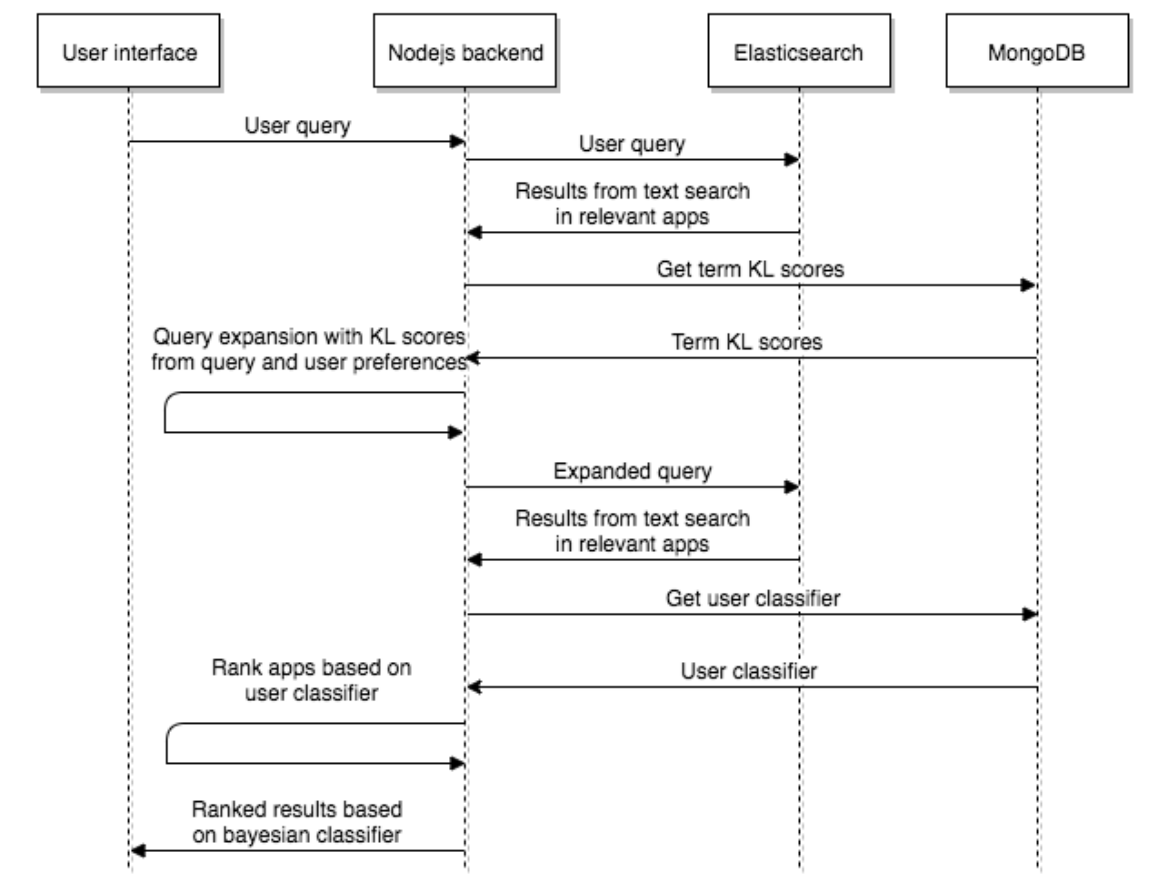
\includegraphics[width=1\linewidth]{img/sequence-diagram-rudihagen.png}
  \caption{Sequence diagram from Rudihagen's implementation of query expansion. Figure taken from \cite{master-thesis}.}
  \label{fig:sequence-diagram-rudihagen}
\end{figure}

[?? need a transition here]
The project report \cite{project-report} describes a query expansion implementation with less round trips,
which were reduced to two roundtrips between the web server and the search engine.
The measured latencies was well within the limit of 100 ms.
An important remark is that all the tests were done locally.
This means that a test setup at a hosting provider would most likely yield significantly higher response times.

The project report had two different implementations, one without query expansion and one with query expansion.
The implementation without query expansion is used as a baseline.
The query expansion implementation had a latency increase of about 2 times compared the baseline implementation.
In a real world environment the increased latency may exceed the 100 ms interactive requirement.

\section{Implementation}
\label{sec:implementation}
Two different platforms were used during the implementation.
The initial implementation used Lucene as the search engine.

\subsection{Algorithm}
[Write introduction pharagraph]
The algorithm used for query expansion is similar on both

The algorithm starts by sending a terms search to the search engine.
From the search engine a results i retrieved

Initially the terms search is sent to the search engine.
The initial search is often called the top-k documents
The photos from the result are then looped through to extract all the tags.
Each tag is stored in an hash map for fast retrieval later.
All the tags are stored together with information about how many occurences each tag have in the top-k documents,
how many terms there are in total in the top-k documents,
how many times the tag appears in the collection,
and how many terms there are in total in the collection.

The information about how many times a tag appears in the collection are retrieved from the search engine.
The number of search engine accesses depends on the number of unique tags in the top-k documents.

After each


\begin{algorithm}
  \begin{algorithmic}
    \Require{Search terms from the user is defined as $searchTerms$}
    \State $initialSearchResult \gets \Call{termsSearch}{searchTerms}$
    \State $termsData \gets [ ]$
    \State $sortedTerms \gets [ ]$

    \For {$photos$ in $initialSearchResult$}
      \For {$term$ in photos}
        \State $numberOfTimesInCollection \gets \Call{getNumberOfTimesInCollection}{term}$
        \State $numberOfTimesInCollection \gets \Call{getNumberOfTimesInCollection}{term}$
        \State \Call{insertTermsData}{term, numberOfTimesInCollection, numberOfTermsInCollection}
      \EndFor
    \EndFor
    \For {$term$ in $termsData$}
      \State $\Call{calulate}$
      \Call{insertTerm}{sortedTerms, term}
    \EndFor

  \end{algorithmic}
  \caption{Algorithm used in the Lucene implementation.}
\end{algorithm}

\subsection{Lucene Architecture}
Most search engines strives to hold the data in memory.
To achieve the performance desired by Lucene the whole index is kept in memory.

The tag field is stored with information about document frequency for each term.
The document frequency is required to calculate the KL score for each term.

Minimal Java optimizations

Even though the Lucen implementation delivered promising results, Lucene in itself is not scalable.
As one of the research questions

\begin{figure}[h!]
  \centering \includegraphics[width=0.9\linewidth]{img/sequence-diagram-lucene.png}
  \caption{Sequence diagram for the Lucene implementation.}
  \label{fig:sequence-diagram-lucene}
\end{figure}

\subsubsection{Indexing}
\subsubsection{Searching}



\subsection{Elasticsearch Architecture}
To acheive the scalability across multiple nodes, the final implementation were done in Elasticsearch.
[?? move to approach?]
Elasticsearch has two different mapping options, dynamic mapping and static mapping.

\subsubsection{Elasticsearch Plugin API}
Elasticsearch has it's own plugin API \footnote{\url{https://www.elastic.co/guide/en/elasticsearch/plugins/5.3/index.html}}.
When a plugin is installed, the installation are done on all the nodes.
The plugin API has two main catogories: core plugins and community contributed plugins.
Core plugins are plugins which are a part of the Elasticsearch project.
These plugins are develop by the Elastic team.
Community contributed plugins, are plugins outside the Elasticsearch project.
These plugins are develop by the community.

The implementation decribed in this report belongs to the community contributed plugins.

The implemented plugin extends the current Elasticsearch REST API.

Architecture with Elasticsearch.

Elasticsearch plugin to extend the Elasticsearch API.

Elasticsearch plugin functionality

\begin{figure}[h!]
\centering 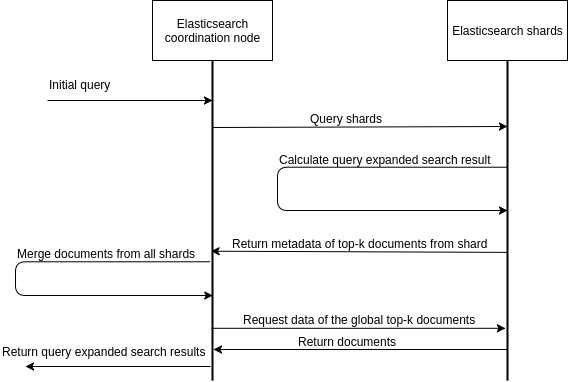
\includegraphics[width=0.9\linewidth]{img/sequence-diagram-elasticsearch.png}
\caption{Sequence diagram for the Elasticsearch implementation.}
\label{fig:sequence-diagram-lucene}
\end{figure}

\subsubsection{Indexing}
\subsubsection{Searching}


\subsection{Web Server}
- Node.js, version
- Configuration NODE\_ENV=production
- pm2
- two endpoints, one for base line one for query expansion
